Pour l'existence d'au moins une solution, via des outils d'analyse, nous allons devoir sortir de l'ensemble des polygones en travaillant avec des objets plus souples, à savoir les \ncycles\ que nous définissons tout de suite.


% ----------------------- %


\begin{defi}
	Pour $n \in \NN_{\geq3}$, un \og \emph{\ncycle} \fg\ désigne une liste ordonnée de $n$ points du plan, les répétitions étant possibles.
	Nous noterons $A_1 A_2 \cdots A_n$ un \ncycle, et appellerons \og \emph{sommets}\fg\ du \ncycle\ les points $A_i$ pour $i \in \ZintervalC{1}{n}$.
\end{defi}


\begin{defi}
    Pour tout \ncycle\ $A_1 A_2 \cdots A_n$, on définit $\big( A^{\,\prime}_i \big)_{i \in \ZZ}$ comme étant $n$-périodique, et vérifiant $A^{\,\prime}_{i} = A_i$ sur $\ZintervalC{1}{n}$.
\end{defi}


\begin{defi}
	Les \og \emph{côtés} \fg\ d'un \ncycle\ $\setproba{L} = A_1 A_2 \cdots A_n$ sont les segments
	$[A^{\,\prime}_i A^{\,\prime}_{i+1}]$ pour $i \in \ZintervalC{1}{n}$,
	et
	la \og \emph{longueur} \fg\ de $\setproba{L}$ est définie par $\cyclelen{\setproba{L}} = \dsum_{i=1}^{n} A^{\,\prime}_i A^{\,\prime}_{i+1}$.
\end{defi}


\begin{defi}
	Un \ncycle\ $\setproba{L} = A_1 A_2 \cdots A_n$ est dit \og \emph{convexe} \fg\ si, pour chaque côté $[A^{\,\prime}_i A^{\,\prime}_{i+1}]$, tous les sommets de $\setproba{L}$ sont dans un même demi-plan fermé délimité par la droite $(A^{\,\prime}_i A^{\,\prime}_{i+1})$ (un sommet peut donc être sur cette droite).
\end{defi}


\begin{defi}
	Un \ncycle\ est \og \emph{dégénéré} \fg\ s'il a, au moins, trois sommets consécutifs alignés.
\end{defi}


\begin{center}
	\small\itshape\centering
	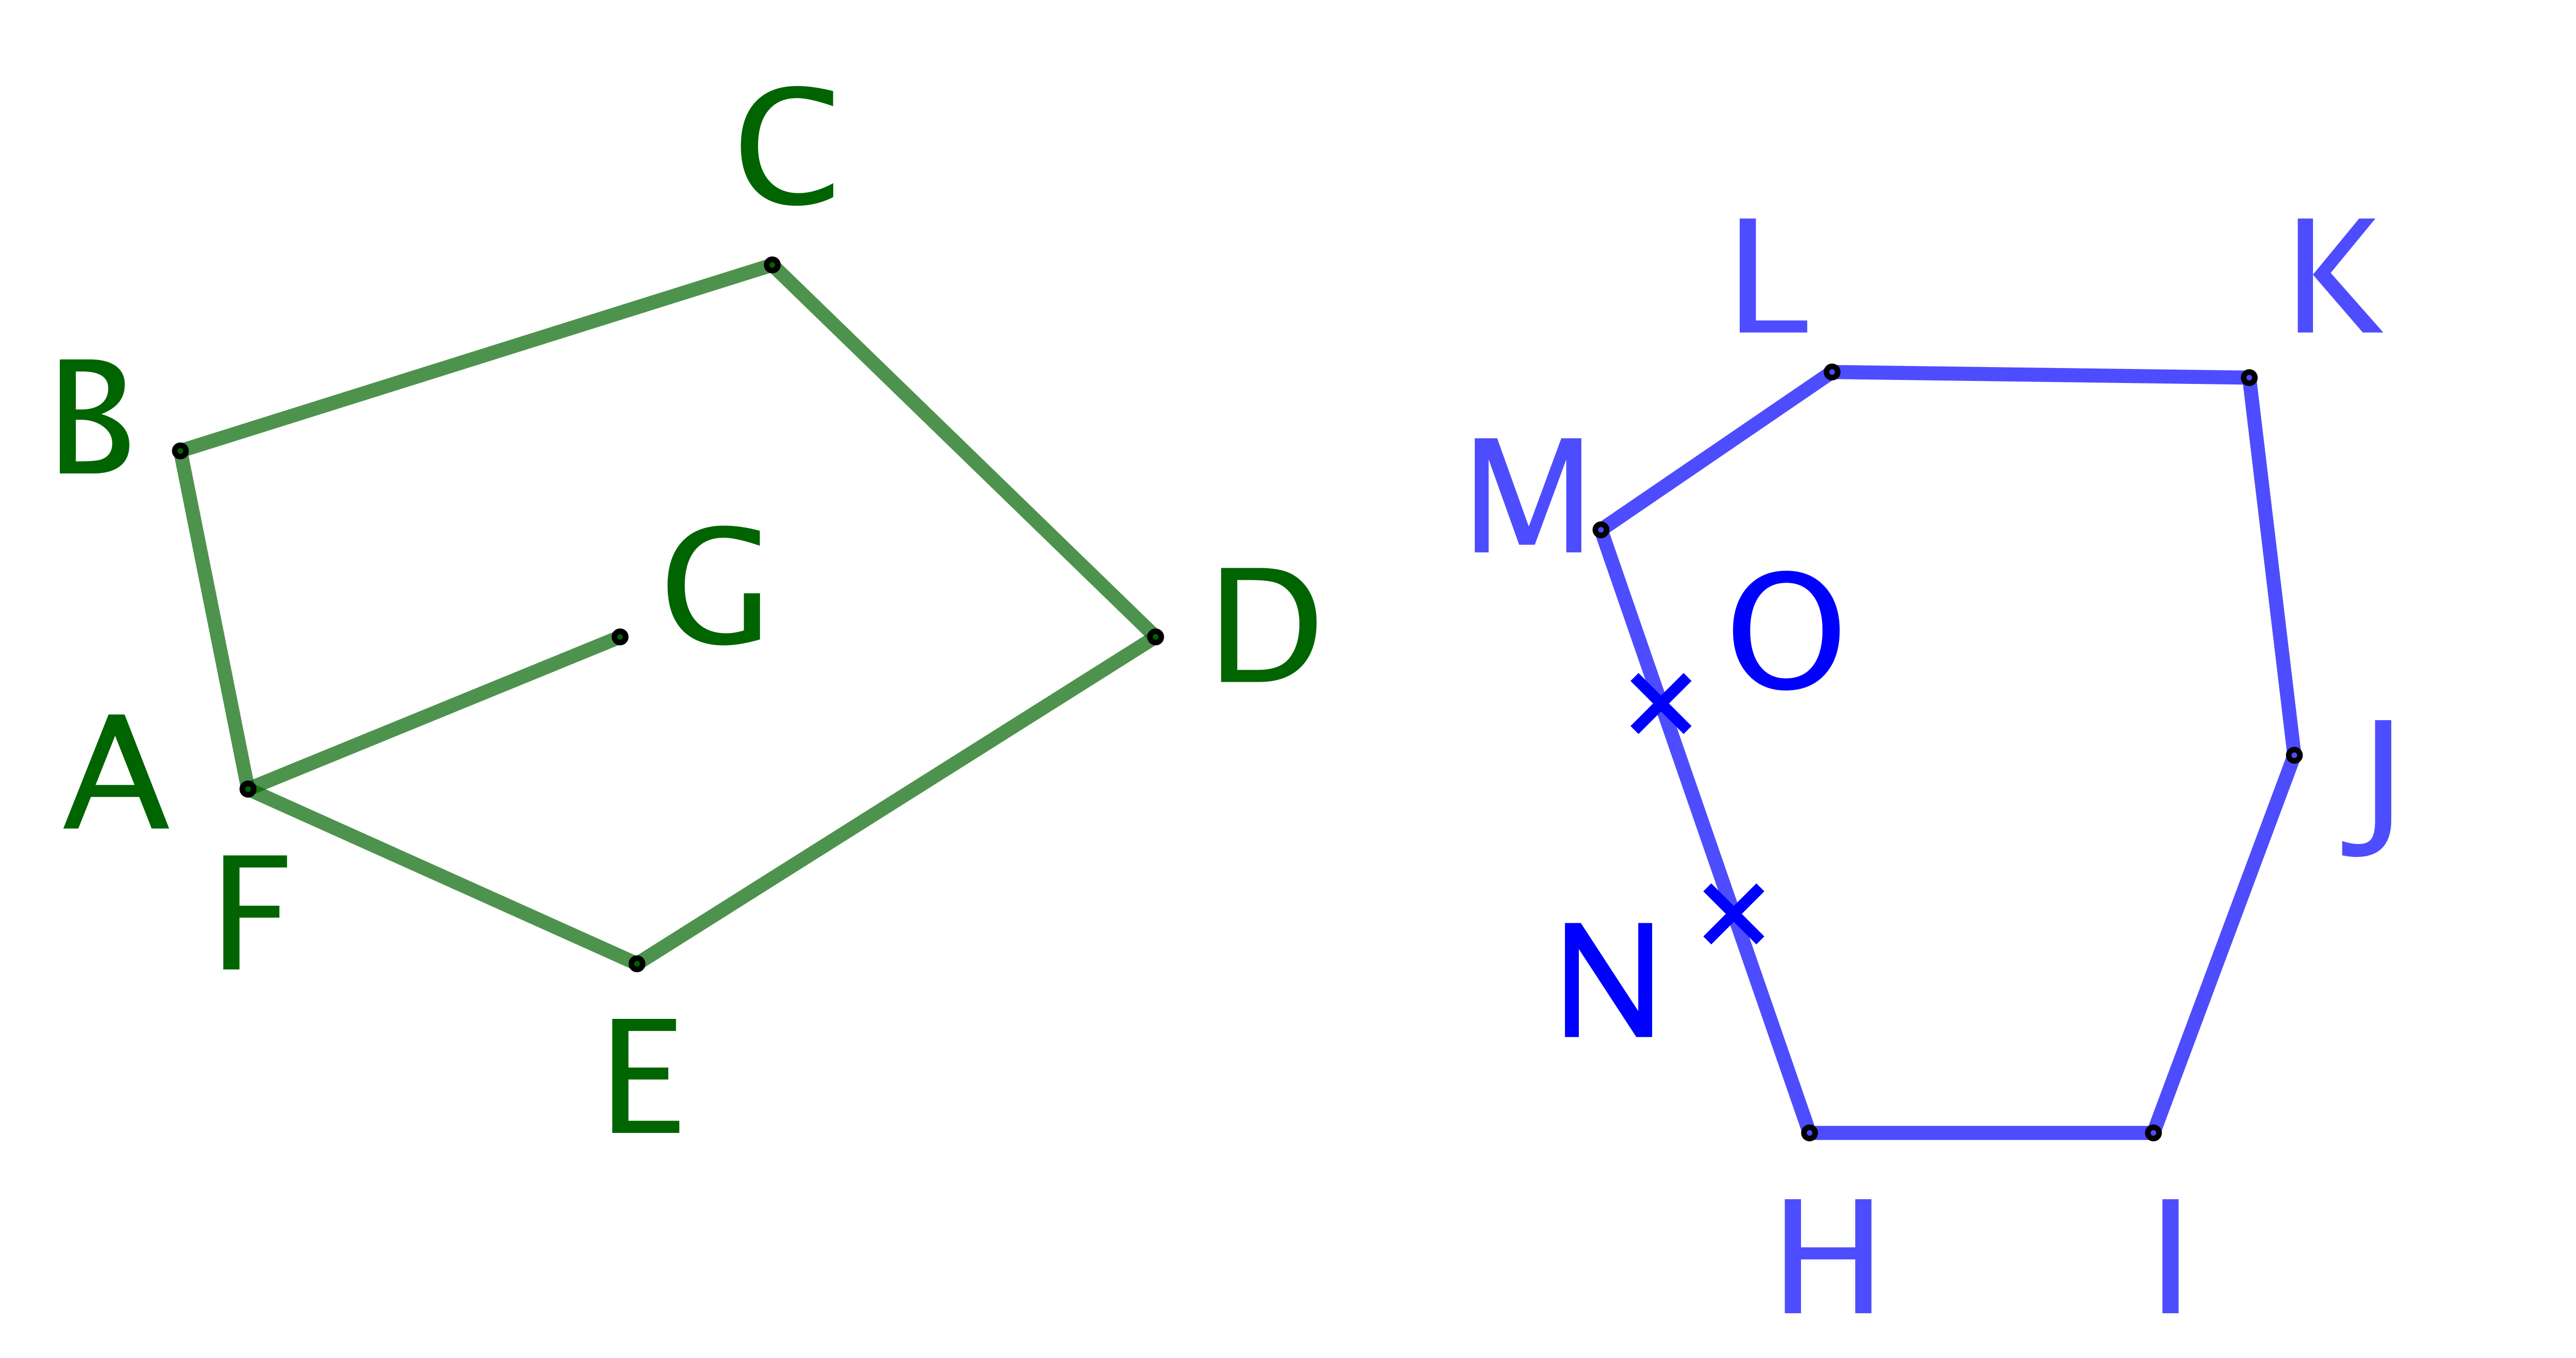
\includegraphics[scale=.35]{content/polygon/def/degenerated-ncycles.png}
	
	\smallskip
	$ABCDEFG$ est un \ncycle\ ni dégénéré, ni convexe.
	
	\smallskip
	$HIJKLMNO$ est un \ncycle\ dégénéré et convexe.
\end{center}


% ----------------------- %


\newpage

\begin{defi}
	Un \og \emph{\ngone} \fg\ $\setproba{P}$ est un \ncycle\ vérifiant les conditions suivantes qui impliquent $n \geq 3$, et que les sommets sont distincts deux à deux.
	%
	\begin{itemize}
		\item Les côtés de $\setproba{P}$ contienne tous exactement deux sommets.

		\item Des côtés non contigus de $\setproba{P}$ ne sont jamais sécants.
	\end{itemize}


	Si certains côtés non contigus sont sécants, mais tous les sommets distincts deux à deux, nous parlerons de \og \emph{\ngone\ croisé} \fg.%
	\footnote{
		Bien retenir que, par définition, un \ngone\ n'est jamais croisé.
		Dès lors, la longueur d'un \ngone\ correspond à son périmètre.
	}
\end{defi}


\begin{defi}
	Un \ngone, croisé ou non, est dit \og \emph{équilatéral} \fg\ si tous ses côtés sont de même mesure.
\end{defi}


\begin{defi}
	Un \ngone, croisé ou non, est dit \og \emph{équiangle} \fg\ si tous ses angles au sommet sont de même mesure.
\end{defi}


\begin{defi}
	Un \ngone, croisé ou non, est dit \og \emph{régulier} \fg\ s'il est à la fois équiangle et équilatéral.
\end{defi}


\begin{remark}
	Un losange non carré est un \nequi\ convexe non régulier, et un rectangle non carré est un \niso\ convexe non régulier.
\end{remark}


\begin{remark}
	Il existe des \nregs\ et croisés.


    \vspace{-1.5em}
    
    \begin{multicols}{2}
    	\small\itshape\centering
    	
	    \null\vfill

	    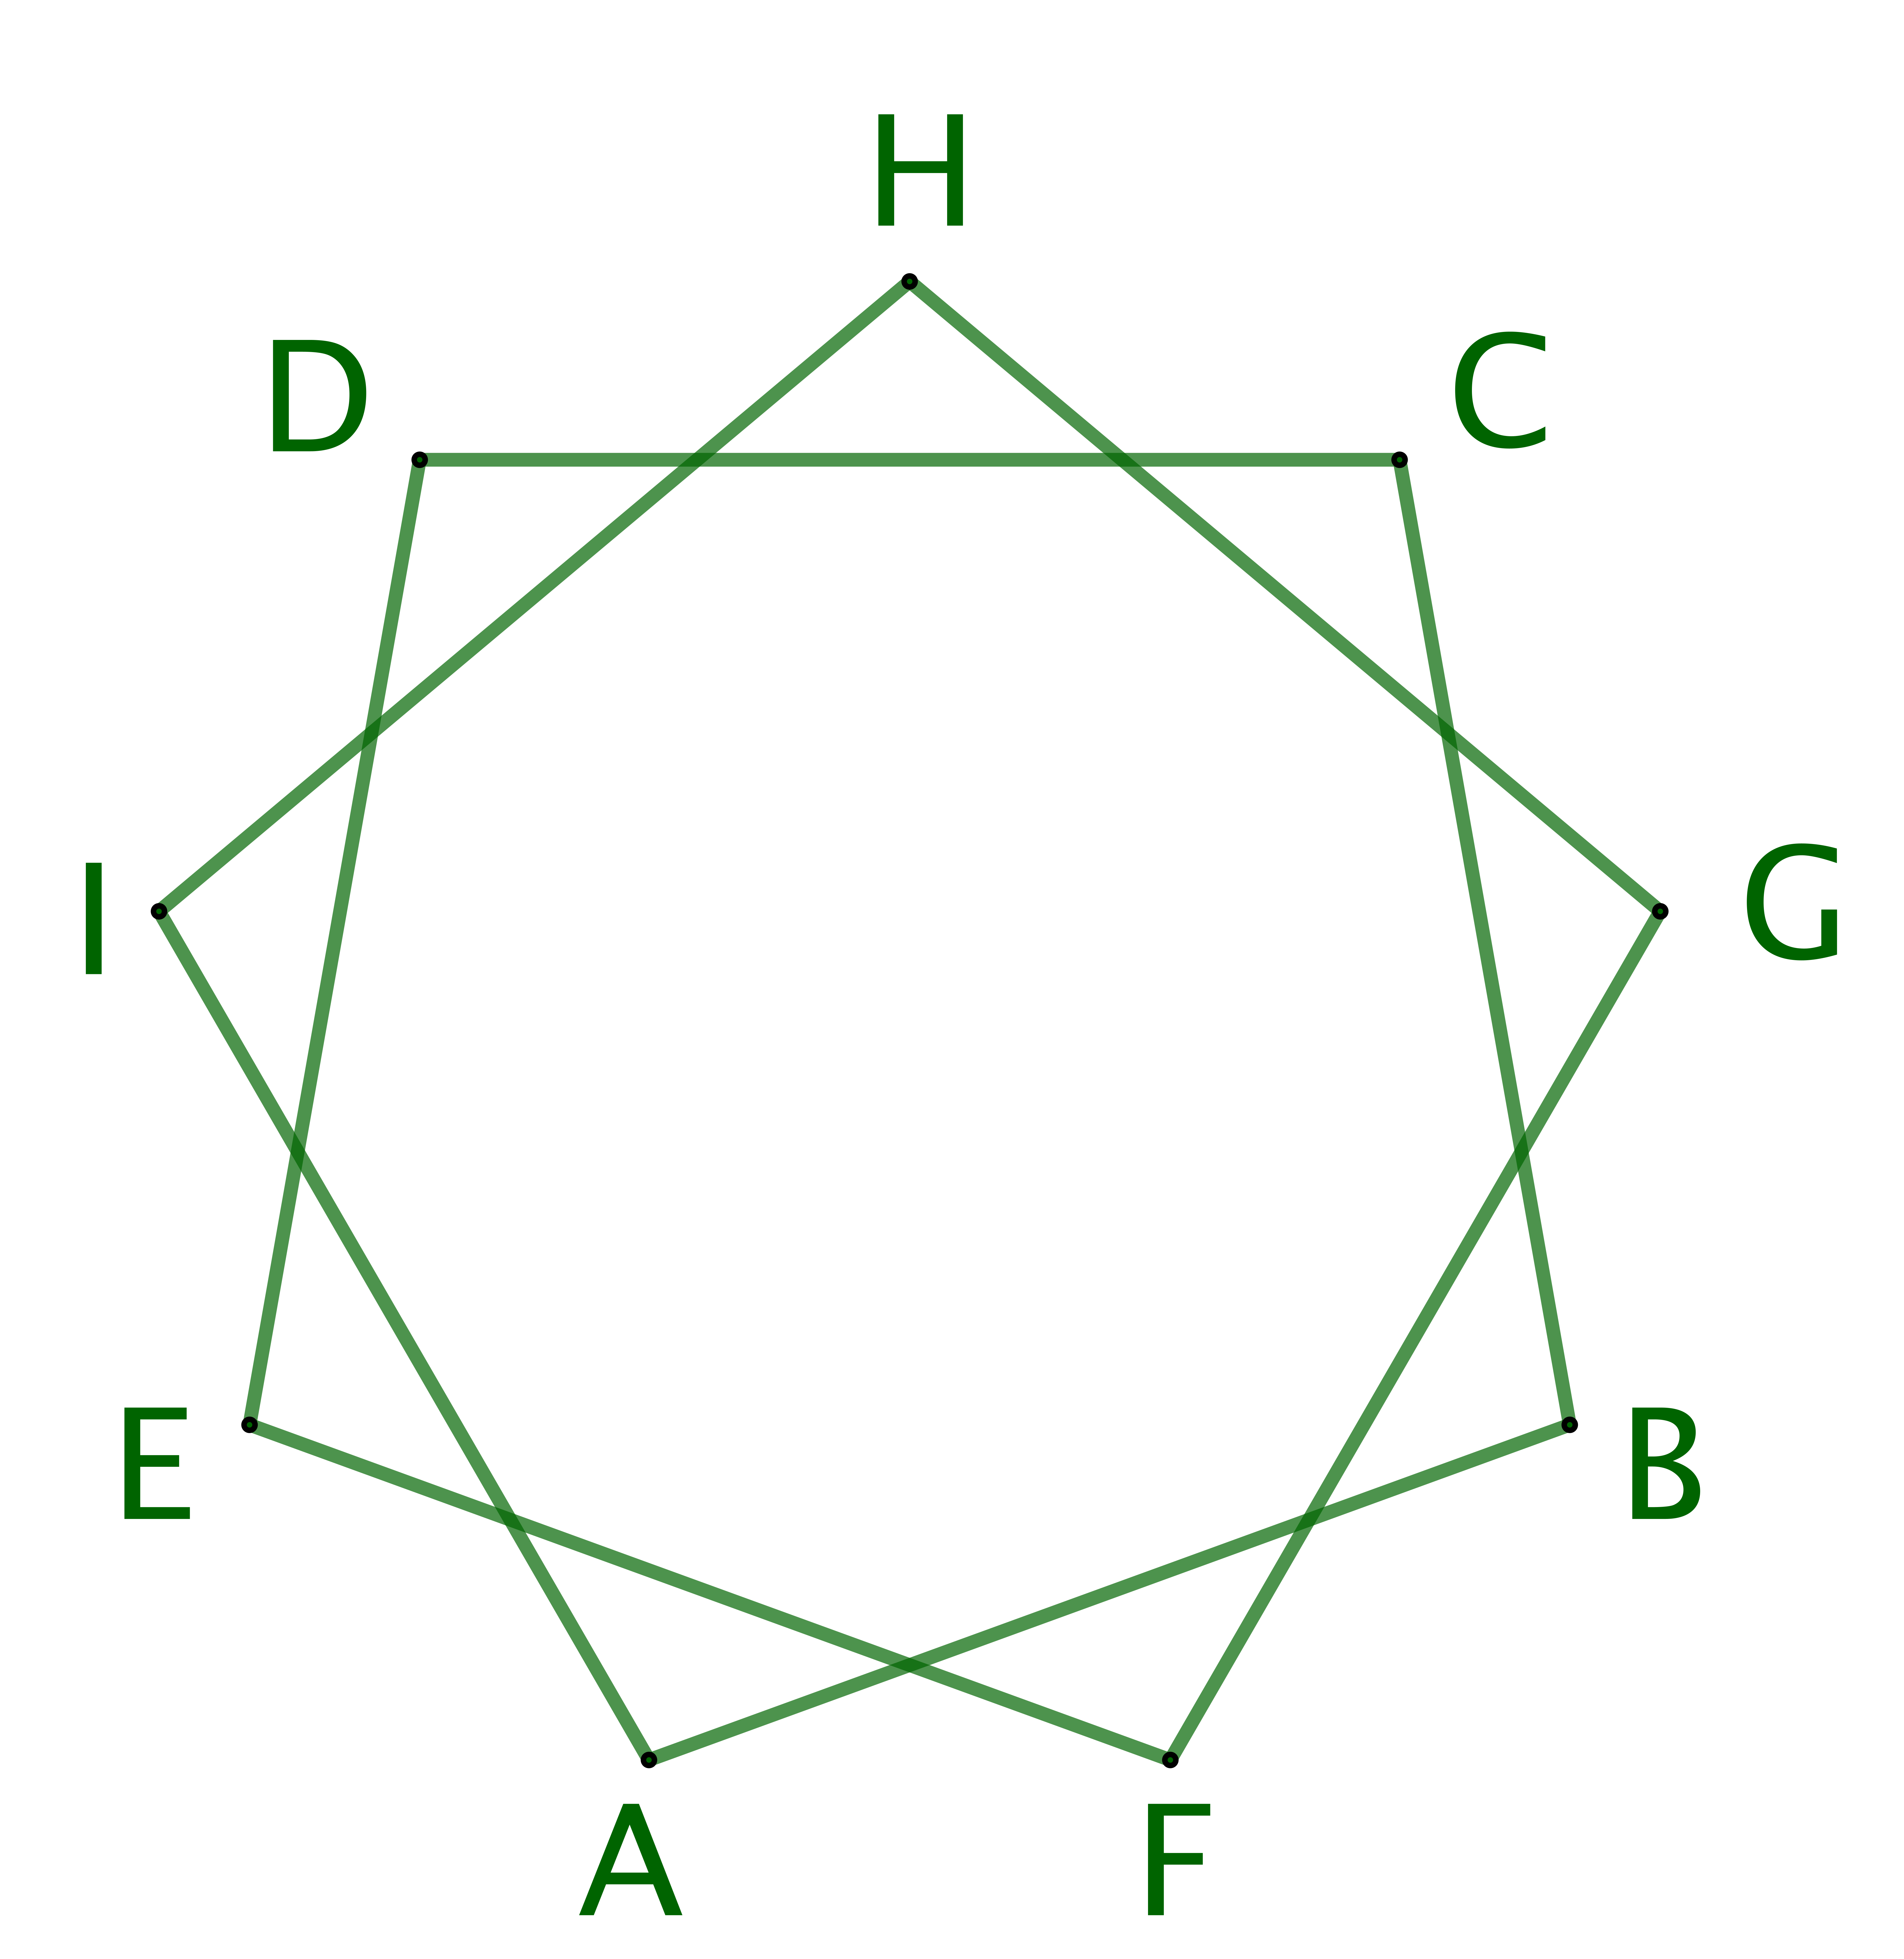
\includegraphics[scale=.175]{content/polygon/def/9-iso-non-conv.png}
    
        \smallskip
        Un ennéagone régulier croisé dit étoilé.%
	    \footnote{
	        La construction se fait via $AFBGCHDIE$ qui est un \xreg{9} convexe. Elle se généralise à tout \nreg\ tel que $n$ soit impair.
	    }

%	    \vfill\null

    	\columnbreak
	
	    \null\vfill
	    
	    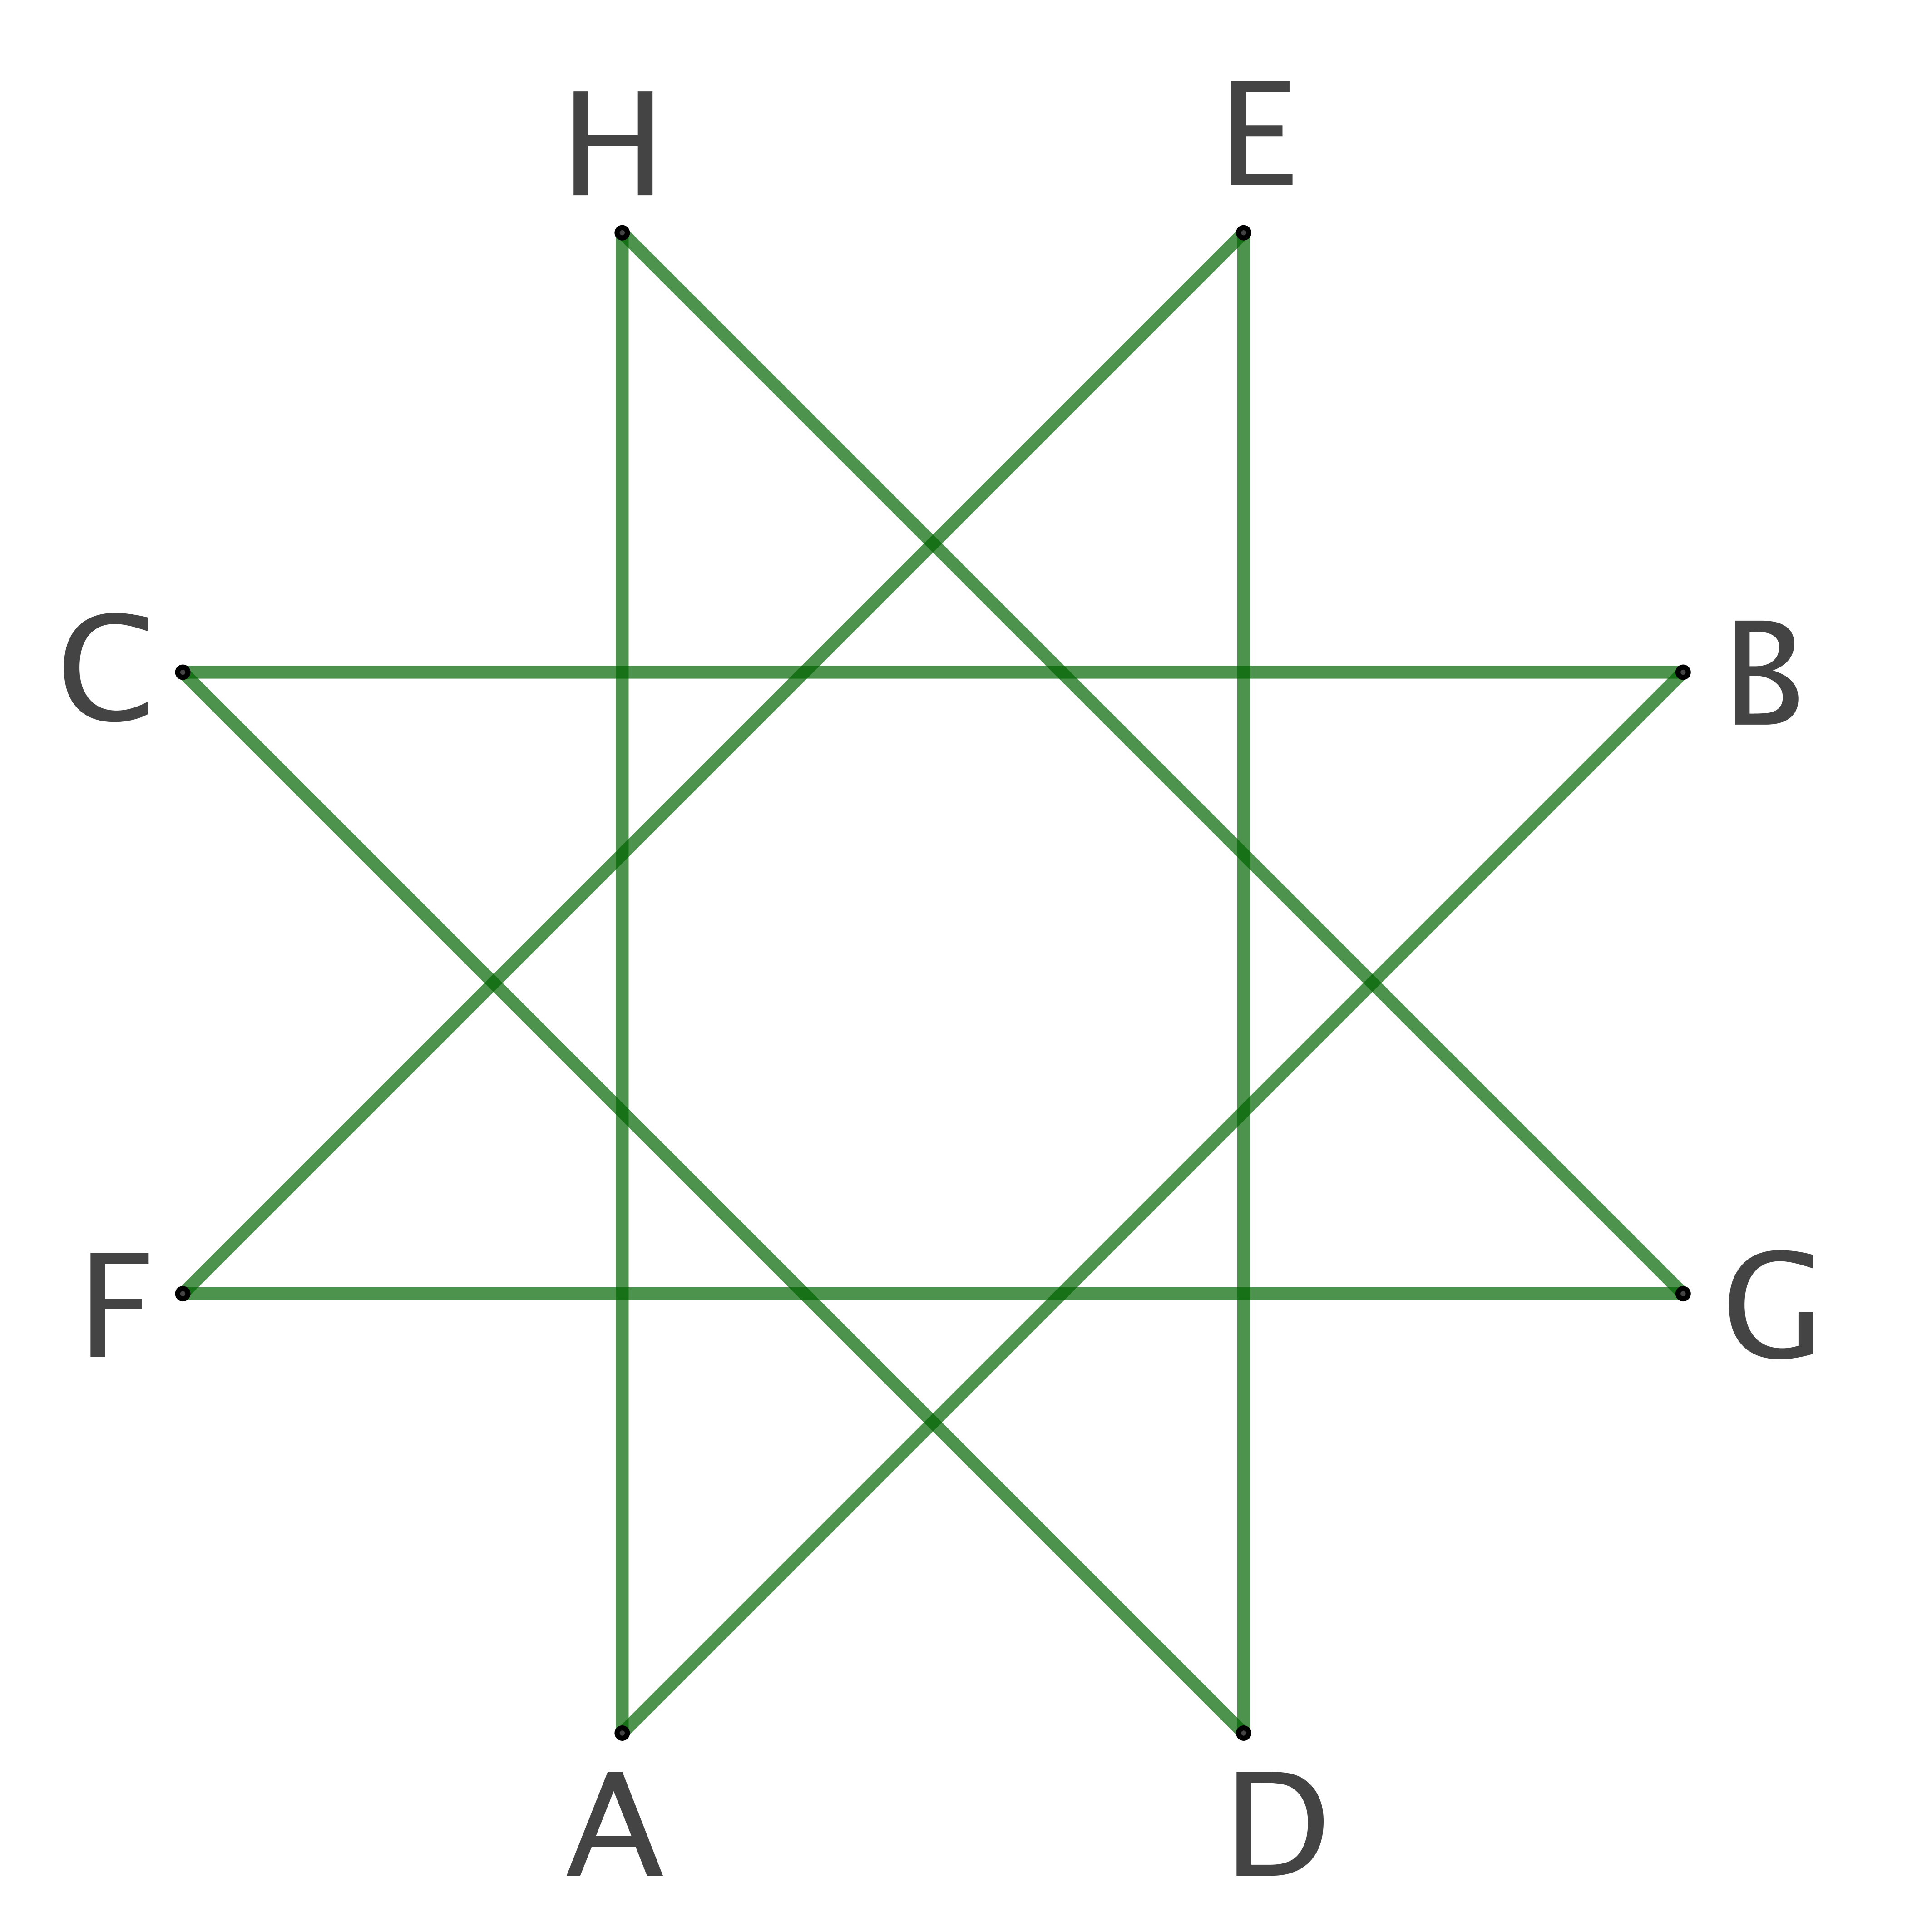
\includegraphics[scale=.3]{content/polygon/def/8-iso-non-conv.png}
    
        \smallskip
        Un octogone régulier croisé dit étoilé.%
	    \footnote{
	        La construction se fait via le \xreg{8} convexe intérieur. Elle se généralise à tout \nreg\ tel que $n$ soit pair.
	    }

%	    \vfill\null
    \end{multicols}
\end{remark}
